\documentclass[xcolor=pdftex,dvipsnames,table,mathserif,aspectratio=169]{beamer}
\usetheme{default}
\usetheme{metropolis}
\usepackage{mathtools}
\setbeamersize{text margin left=.3in,text margin right=.3in} 

\usepackage[english]{babel}
\usepackage{pgf,pgfarrows,pgfnodes,pgfautomata,pgfheaps}
\usepackage{amsmath,amssymb,setspace,centernot}
\usepackage[latin1]{inputenc}
\usepackage{pgf,tikz}
\usepackage[T1]{fontenc}
\usepackage{relsize}
\usepackage{pdfpages}
\usepackage[absolute,overlay]{textpos} 
\usepackage{hyperref}
\hypersetup{
    urlcolor=cyan,
}

\DeclareMathOperator*{\argmax}{arg\,max}
\DeclareMathOperator*{\argmin}{arg\,min}

\newcommand{\X}{\mathtt{X}}
\newcommand{\Y}{\mathtt{Y}}

%\newcommand{\R}{\mathbb{R}}
%\newcommand{\E}{\mathbb{E}}
%\newcommand{\V}{\mathbb{V}}
\newcommand{\p}{\mathbb{P}}
\newcommand*\df{\mathop{}\!\mathrm{d}}
\newcommand{\del}{\partial}


% imports
\usepackage{xargs}
\usepackage{xpatch}
\usepackage{etoolbox}
\usepackage{pdflscape}
\usepackage{booktabs}
\usepackage{threeparttable}
\usepackage[skip=0.2\baselineskip]{caption}

% command for inputting raw latex
\makeatletter
\newcommand\primitiveinput[1]{\@@input #1 }
\makeatother

% common table command
\newcommandx{\tablecontent}[4]{
    \begin{threeparttable}[!ht]
        \centering
        \caption{#3}
        \vspace{-1em}
        \footnotesize
        \begin{tabular}{#1}
            \primitiveinput{../tables/#2.tex}
        \end{tabular}
        \vspace{-0.2em}
        \begin{tablenotes}[flushleft]
            #4
        \end{tablenotes}
    \end{threeparttable}
}




% \usepackage{slashbox}
\title{ Advanced Panel Data:\\
Two-way FE and Diff-in-Diff}
\author{Chris Conlon }
\institute{NYU Stern }


\newcommand{\norm}[1]{\left\lVert#1\right\rVert}
\newcommand{\R}{\mathbb{R}}
\newcommand{\E}{\mathbb{E}}
\newcommand{\V}{\mathbb{V}}
\newcommand{\ol}{\overline}
%\newcommand{\ul}{\underline}
\newcommand{\pp}{{\prime \prime}}
\newcommand{\ppp}{{\prime \prime \prime}}
\newcommand{\policy}{\gamma}


\newcommand{\fp}{\frame[plain]}

\date{\today}

\begin{document}
\maketitle

\section*{Staggered TWFE Designs}

\begin{frame}
\frametitle{Staggered TWFE Designs}
A very common method is the following:
\begin{align*}
y_{it} = x_{it} \beta + \tau\cdot  D_{it} + \eta_i + \lambda_t + \varepsilon_{it}
\end{align*}

\begin{itemize}
\item e.g. Different states $i$ enact a policy $D_{it}=1$ in different years $t$.
\item We call this ``staggered'' if not every entity is treated at the same time.
\item Surely this is better than:
\begin{itemize}
\item Single treated state (usual DiD)
\item Contemporaneous role out (can't separate $\tau$ and $\lambda_t$).
\end{itemize}
\item But what does $\tau$ or $\tau_{it}$ actually measure?
\end{itemize}
\end{frame}


\begin{frame}
\frametitle{Literature}
This is part of a rapidly growing literature
\begin{itemize}
\item \href{https://www.sciencedirect.com/science/article/pii/S0304407620303948}{Callaway and Sant'Anna (2020)}
\item \href{http://goodman-bacon.com/pdfs/ddtiming.pdf}{Goodman-Bacon (2021)}
\item \href{https://www.aeaweb.org/articles?id=10.1257/aer.20181169}{de Chaisemartin and D'Haultfoeulle (2020}
\item \href{https://arxiv.org/abs/1804.05785}{Sun and Abraham (2020)}
\item \href{https://bcallaway11.github.io/did/}{R Vignette}
\end{itemize}
\end{frame}


\begin{frame}{Recap: Regular DiD}
\begin{align*}
Y_{it} &= D_i  \cdot Y_{it}(1) - (1-D_i)\cdot  Y_{it}(0), \quad Y_{i,t-1} = Y_{i,t-1}(0)\\
y_{it} &= \alpha + \gamma_i \cdot D_i + \lambda_t \cdot \text{Post}_t +  \alert{\tau  \cdot D_i \times \text{Post}_t }+ \varepsilon_{it}
\end{align*}
\begin{itemize}
\item Nobody treated at $t-1$ and some people treated at $t$.
\item Parallel trends $\mathbb{E}[Y_{it}(0) - Y_{i,t-1}(0) | D_{it}=1] =\mathbb{E}[Y_{it}(0) - Y_{i,t-1}(0) | D_{it}=0]$
\item If parallel trends holds: $\tau = ATT = \mathbb{E}[Y_{it} - Y_{i,t-1} | D_{it}=1]-\mathbb{E}[Y_{it} - Y_{i,t-1} | D_{it}=0]  $
\end{itemize}
\end{frame}

\begin{frame}{Simple Question?}
When does TWFE deliver the $ATT=\mathbb{E}[\tau_{it} | D_{it}=1]$?
\begin{align*}
y_{it} = x_{it} \beta + \tau_{it} \cdot  D_{it} + \eta_i + \lambda_t + \varepsilon_{it}
\end{align*}
\begin{itemize}
\item Only two periods with $D_{i0}=0$ for all $i$.
\item  Constant treatment effects $\tau_{it} = \tau$.
\item Otherwise mostly no...
\end{itemize}
\end{frame}

\begin{frame}{What are we comparing}
\begin{align*}
y_{it} = x_{it} \beta + \tau_{it} \cdot  D_{it} + \eta_i + \lambda_t + \varepsilon_{it}
\end{align*}
Three different control groups when we compare $Y_{it} | D_{it}=1$:
\begin{enumerate}
\item Units that \alert{never get treated}
\item Units that \alert{will be treated later}: $t' > t$
\item But \alert{previously treated units} enter your control group [bad!]
\end{enumerate}
How $\tau_{it}$ varies over time for different \alert{cohorts} will now affect an estimate of $\tau$.
\end{frame}


\begin{frame}{What do we get? (Goodman-Bacon 2020)}
\centering
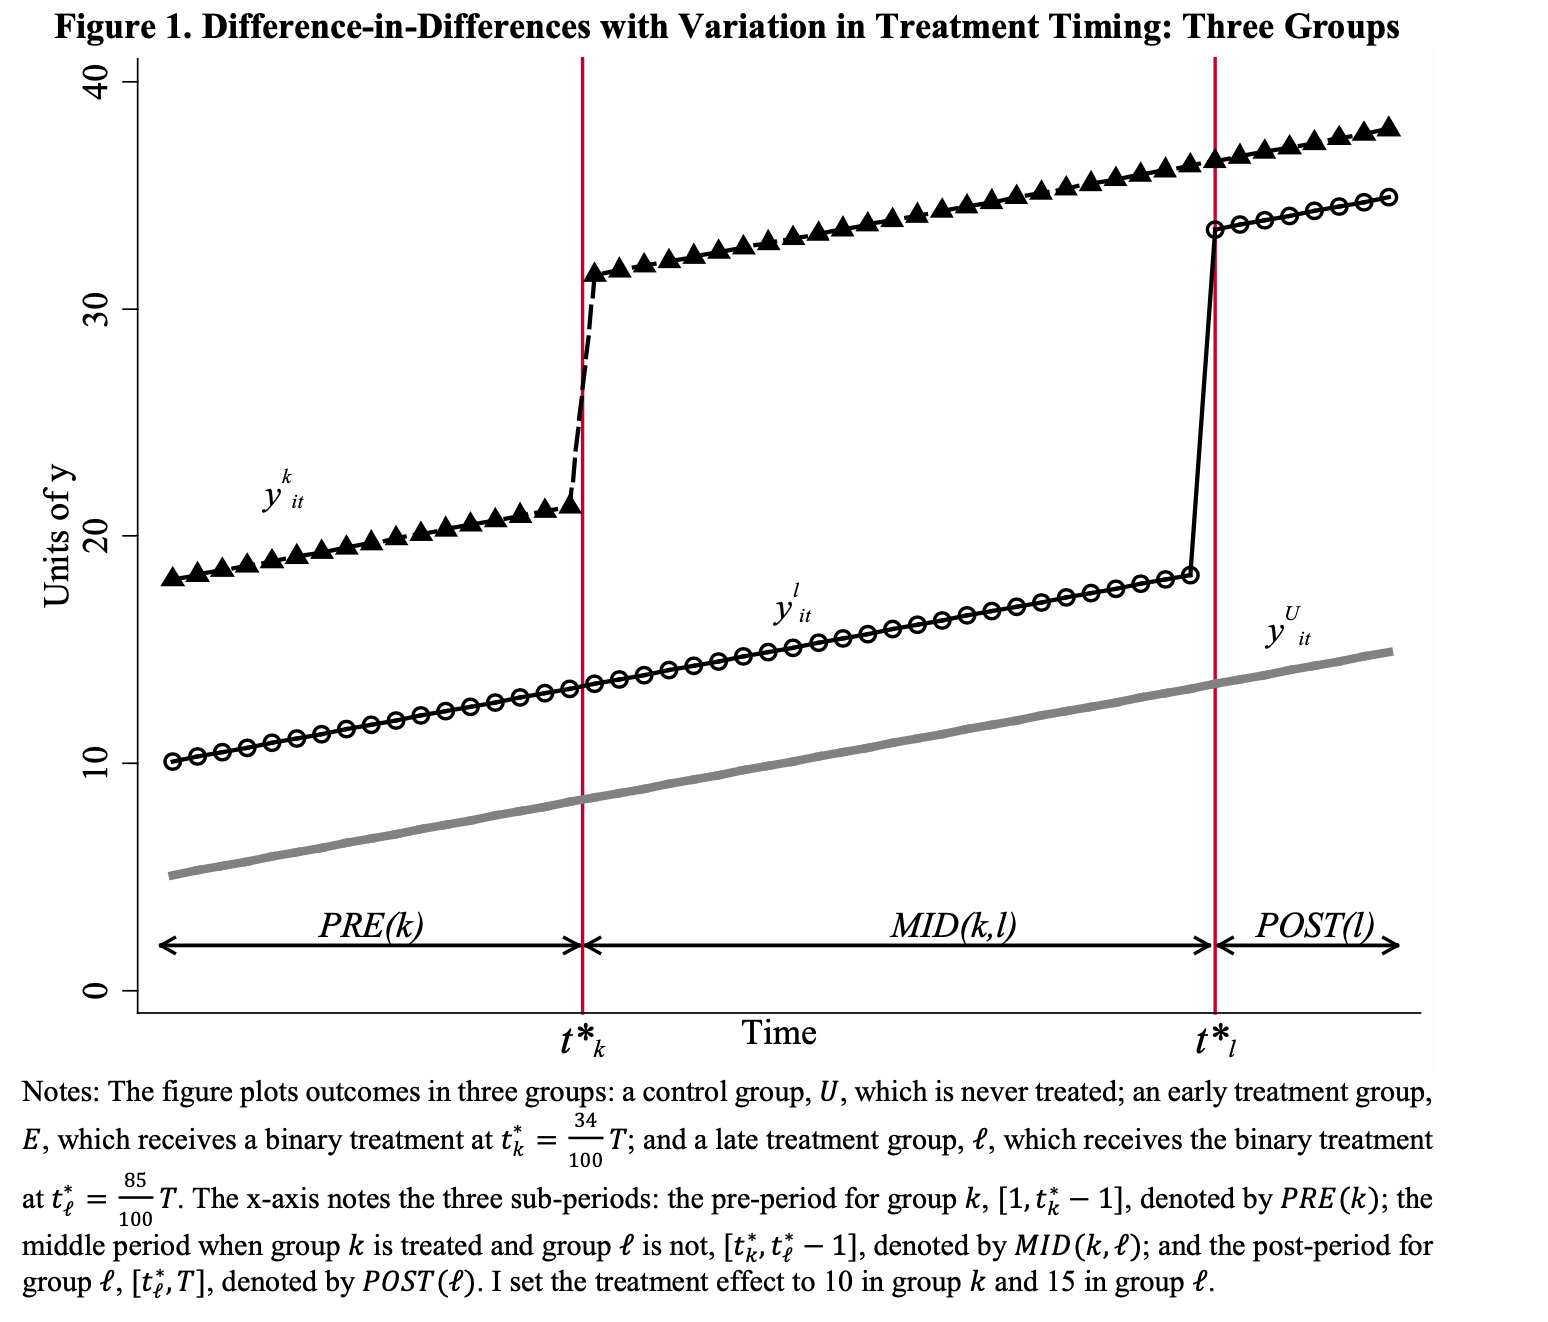
\includegraphics[height=0.9\textheight]{resources/gb_fig1.png}
\end{frame}


\begin{frame}{What do we get? (Goodman-Bacon 2020)}
One thing we might want to know is whether our TWFE estimate of $\widehat{\tau}$ is at all useful.\\
AKA what did we just estimate?
\begin{itemize}
\item Suppose there are two groups $G$ of different treatment timings: \{early, late \}.
\item Think about every possible $2 \times 2$ DD estimate.
\begin{itemize}
\item Early group vs. never treated
\item Late group vs. never treated
\item Early group vs. late group before $t*$
\item Late group vs. early group after $t*$.
\end{itemize}
\end{itemize}
\end{frame}


\begin{frame}{What do we get? (Goodman-Bacon 2020)}
\centering
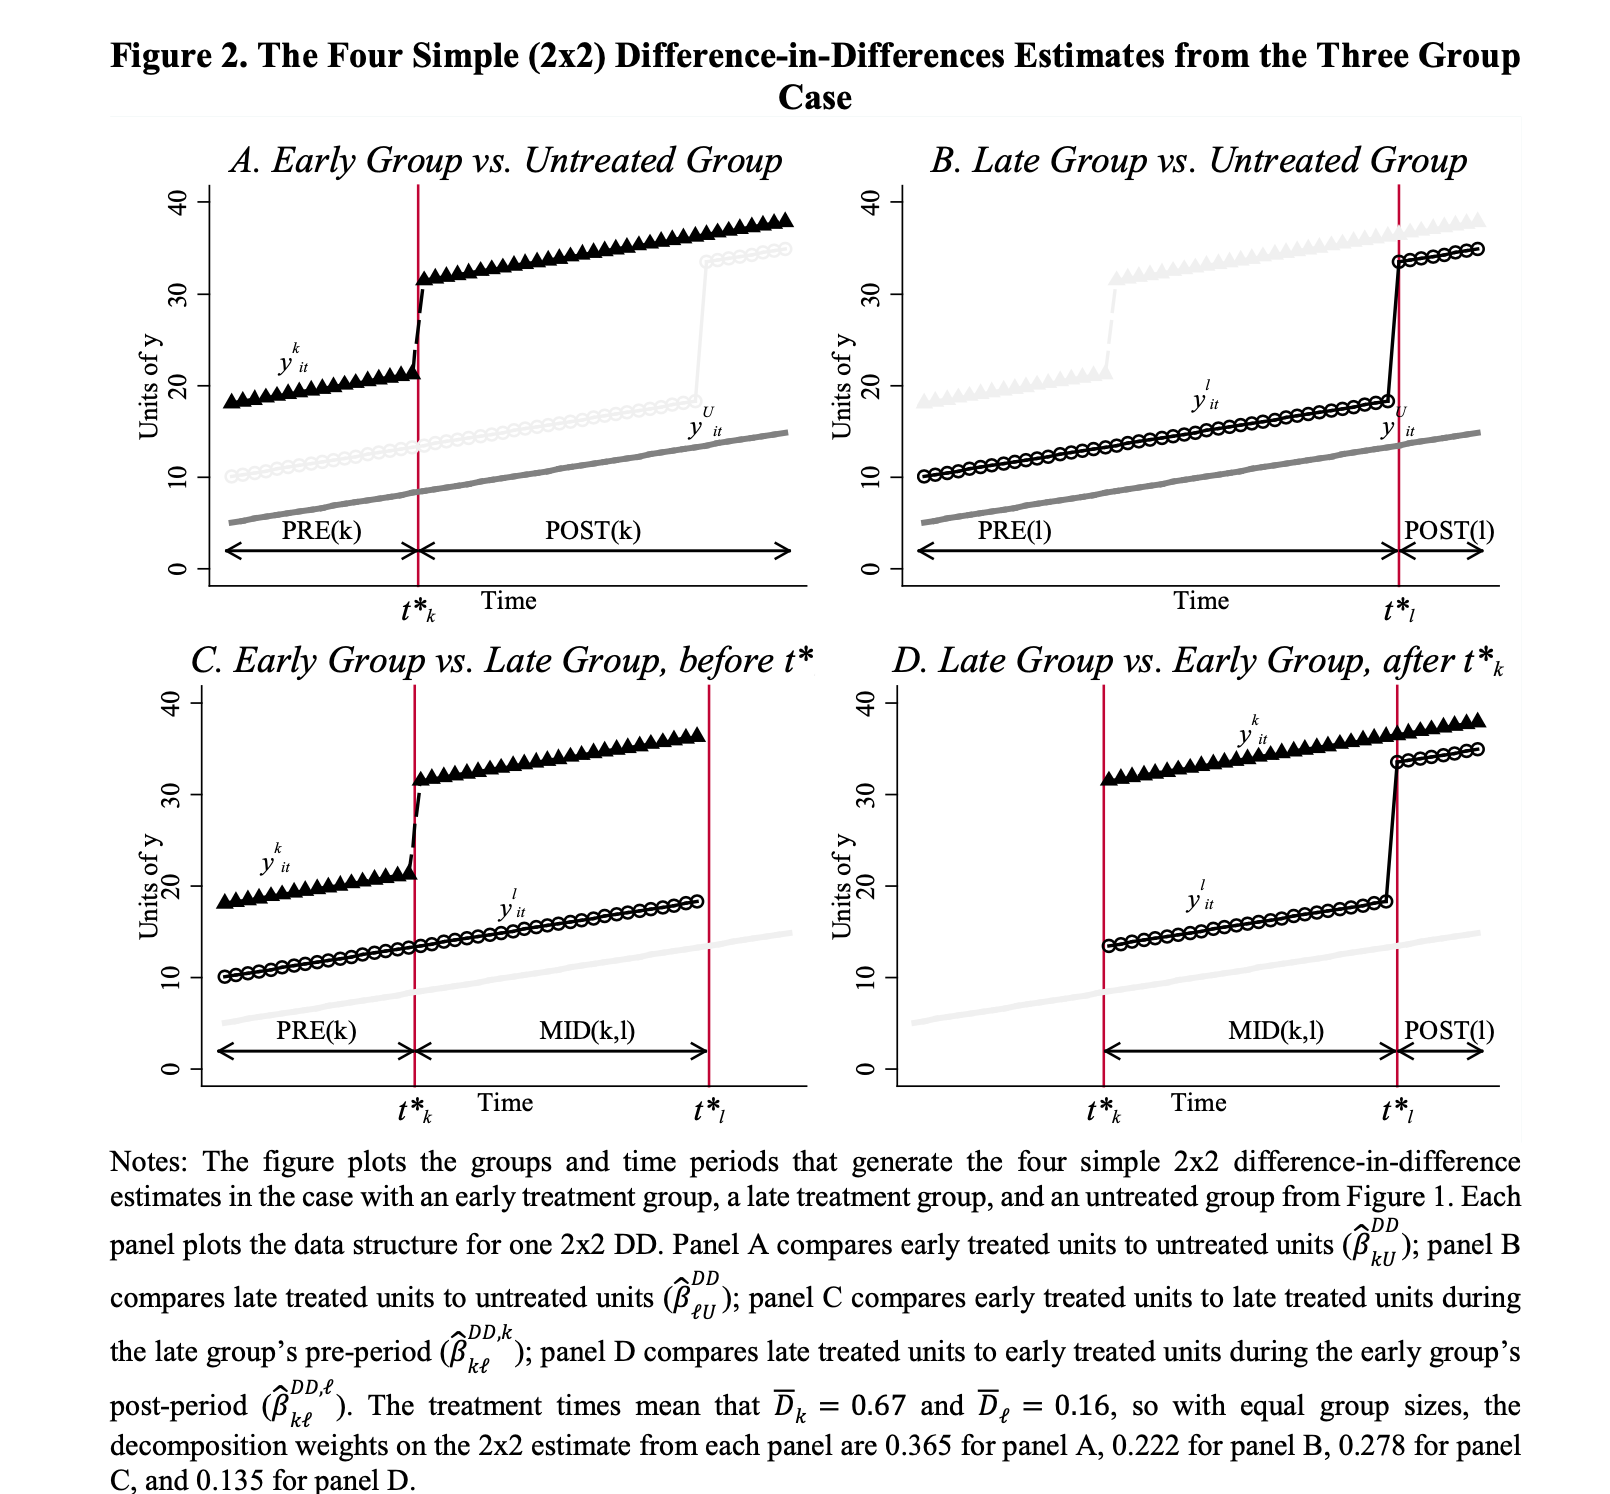
\includegraphics[height=0.9\textheight]{resources/gb_fig2.png}
\end{frame}

\begin{frame}{What do we get? (Goodman-Bacon 2020)}
\begin{align*}
\widehat{\tau}^{D D}&=\sum_{k \neq U} s_{k U} \widehat{\tau}_{k U}+\sum_{k \neq U} \sum_{\ell>k}\left[s_{k \ell}^{k} \widehat{\tau}_{k \ell}^{ k}+s_{k \ell}^{\ell} \widehat{\tau}_{k \ell}^{\ell}\right]\\
\widehat{\tau}_{k U}^{2 x 2} &\equiv\left(\bar{y}_{k}^{P O S T(k)}-\bar{y}_{k}^{P R E(k)}\right)-\left(\bar{y}_{U}^{P O S T(k)}-\bar{y}_{U}^{P R E(k)}\right) \\
\widehat{\tau}_{k \ell}^{2 x 2, k} &\equiv\left(\bar{y}_{k}^{M I D(k, \ell)}-\bar{y}_{k}^{P R E(k)}\right)-\left(\bar{y}_{\ell}^{M I D(k, \ell)}-\bar{y}_{\ell}^{P R E(k)}\right) \\
\widehat{\tau}_{k \ell}^{2 x 2, \ell} &\equiv\left(\bar{y}_{\ell}^{P O S T(\ell)}-\bar{y}_{\ell}^{M I D(k, \ell)}\right)-\left(\bar{y}_{k}^{P O S T(\ell)}-\bar{y}_{k}^{M I D(k, \ell)}\right)
\end{align*}
Corresponding set of weights $s_{k,\ell}$ which depend on size and variance of each group.\\
Variance is largely about how concentrated $D_{it}$ is within each group.
\end{frame}

\begin{frame}{Assuming Equal Groups (Goodman-Bacon 2020)}
\centering
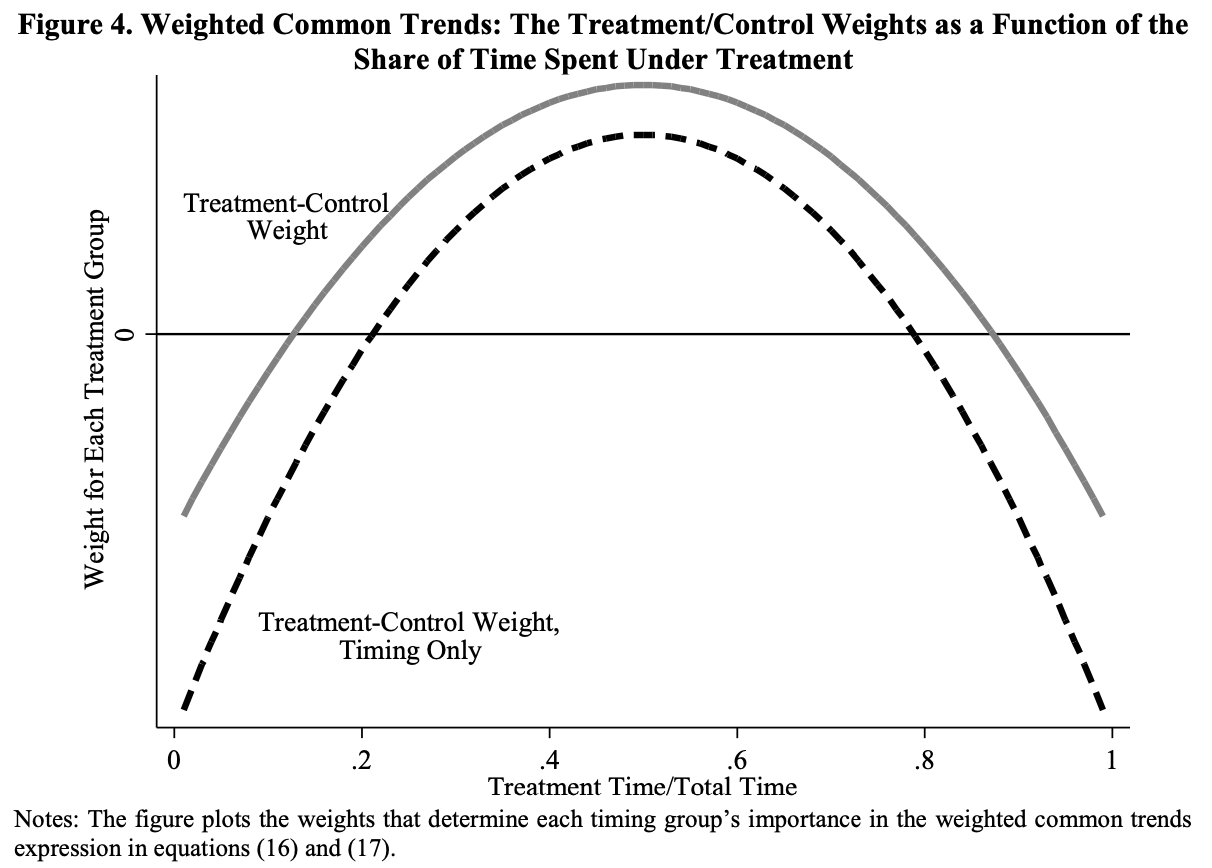
\includegraphics[height=0.9\textheight]{resources/gb_fig4.png}
\end{frame}


\begin{frame}{Time varying TE $\tau_{it}$ (Goodman-Bacon 2020)}
\centering
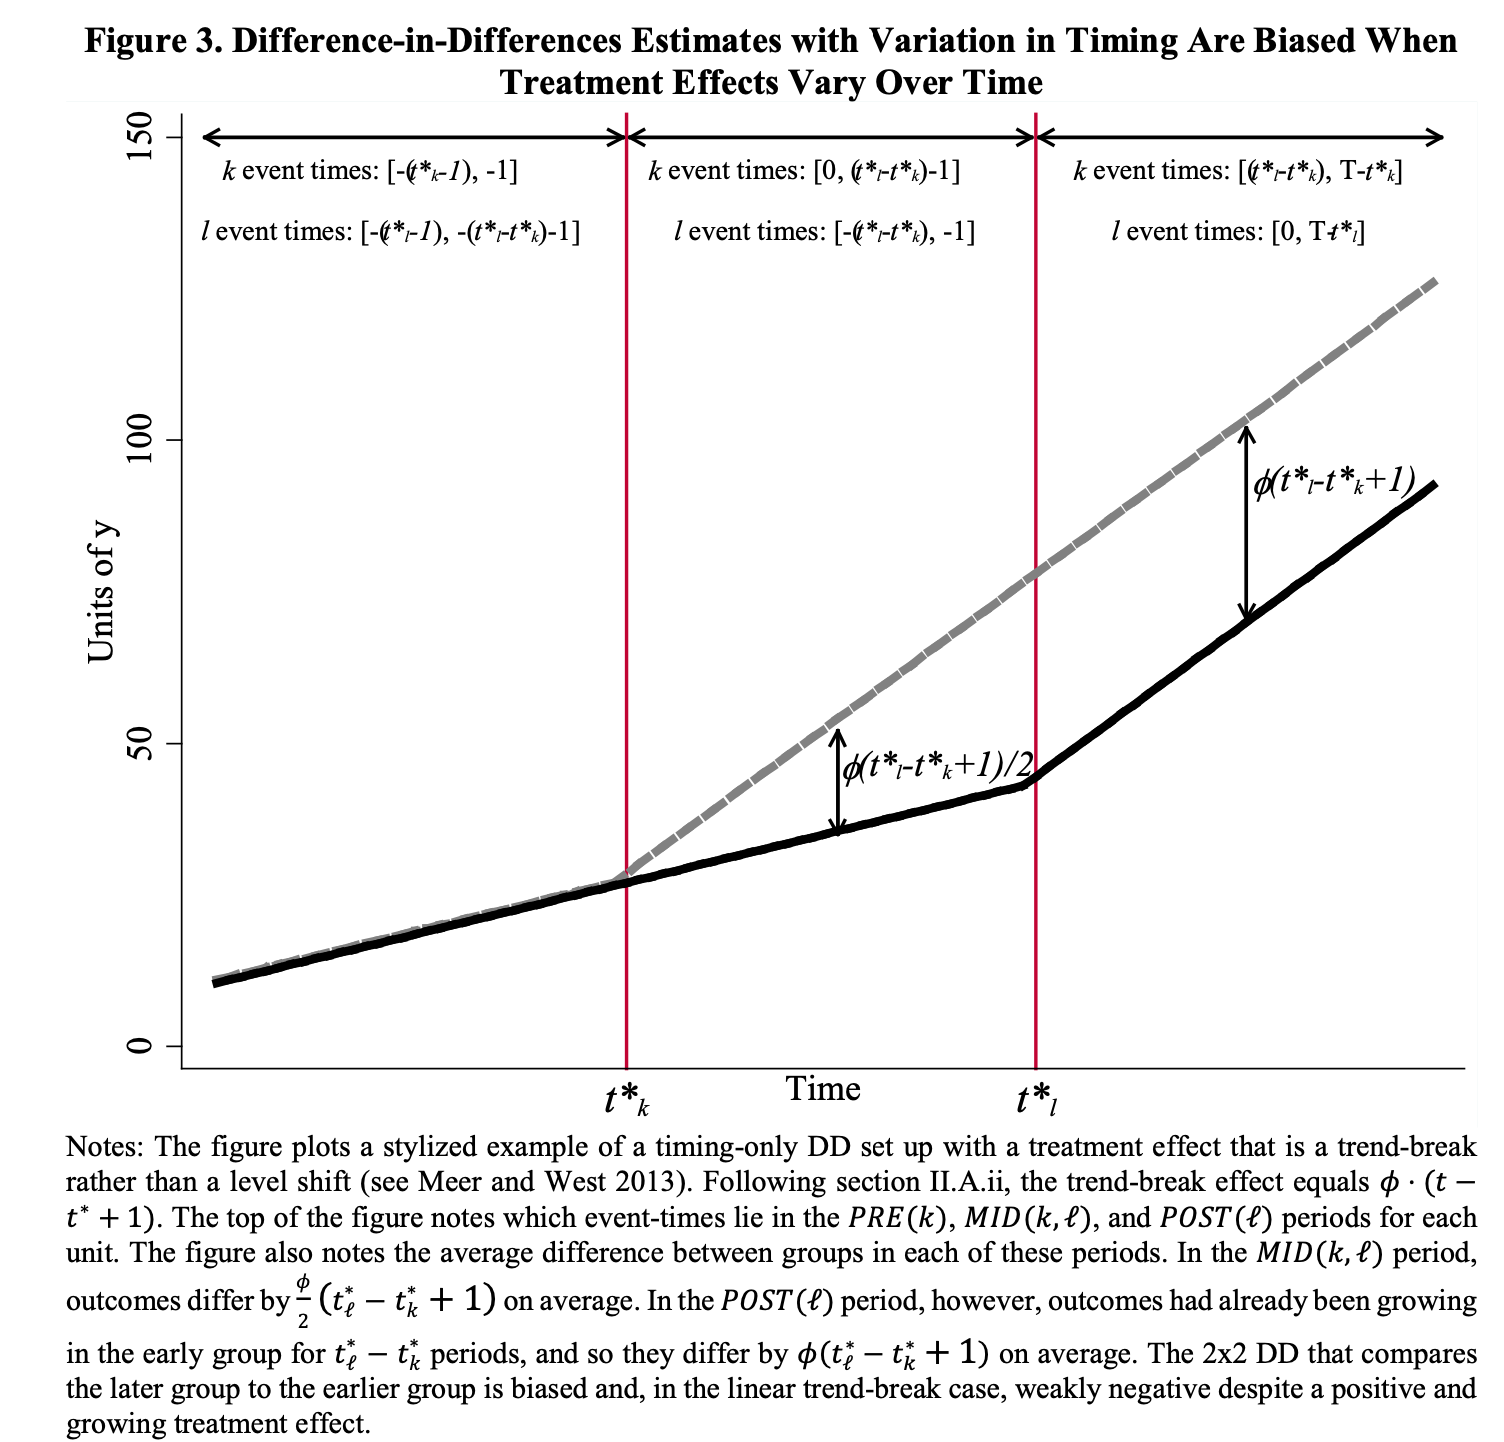
\includegraphics[height=0.9\textheight]{resources/gb_fig3.png}
\end{frame}


\begin{frame}{Application: (Goodman-Bacon 2020)}
\centering
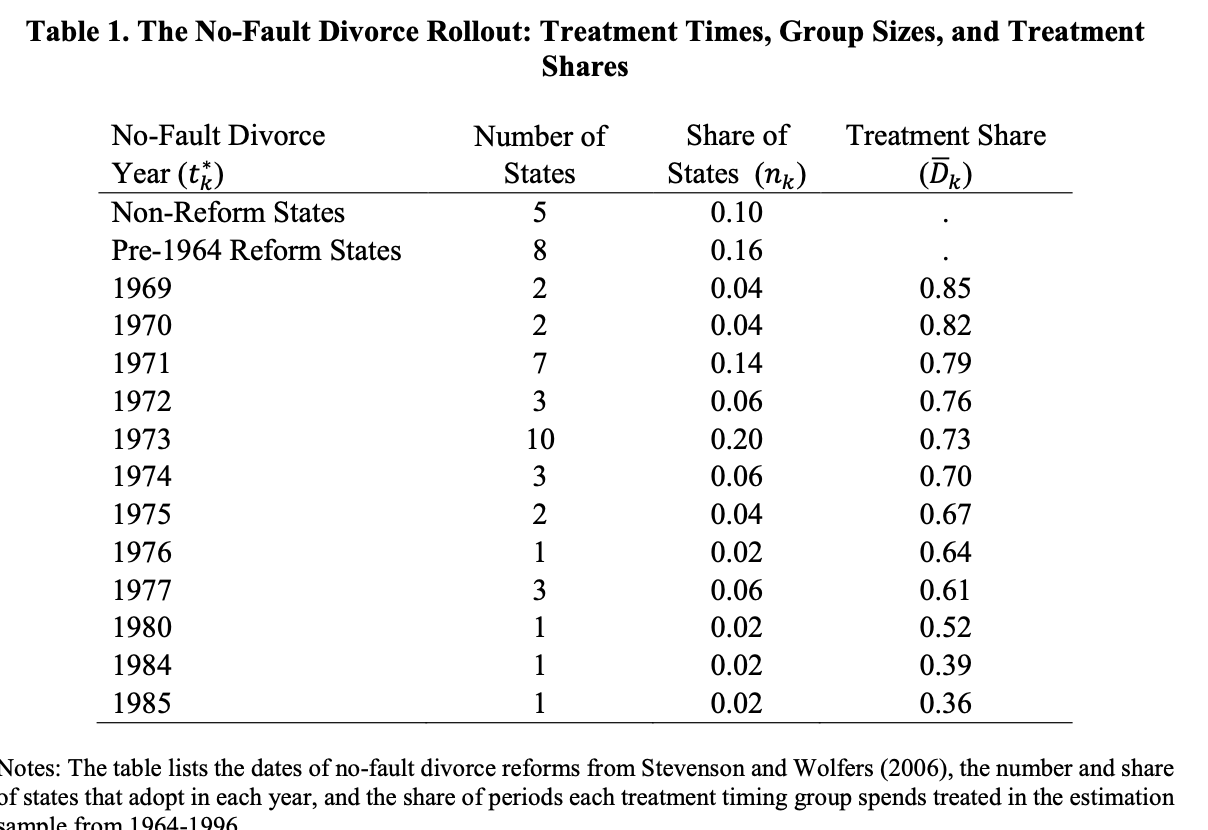
\includegraphics[height=0.9\textheight]{resources/gb_tab1.png}
\end{frame}


\begin{frame}{Event Study Plot (Goodman-Bacon 2020)}
\centering
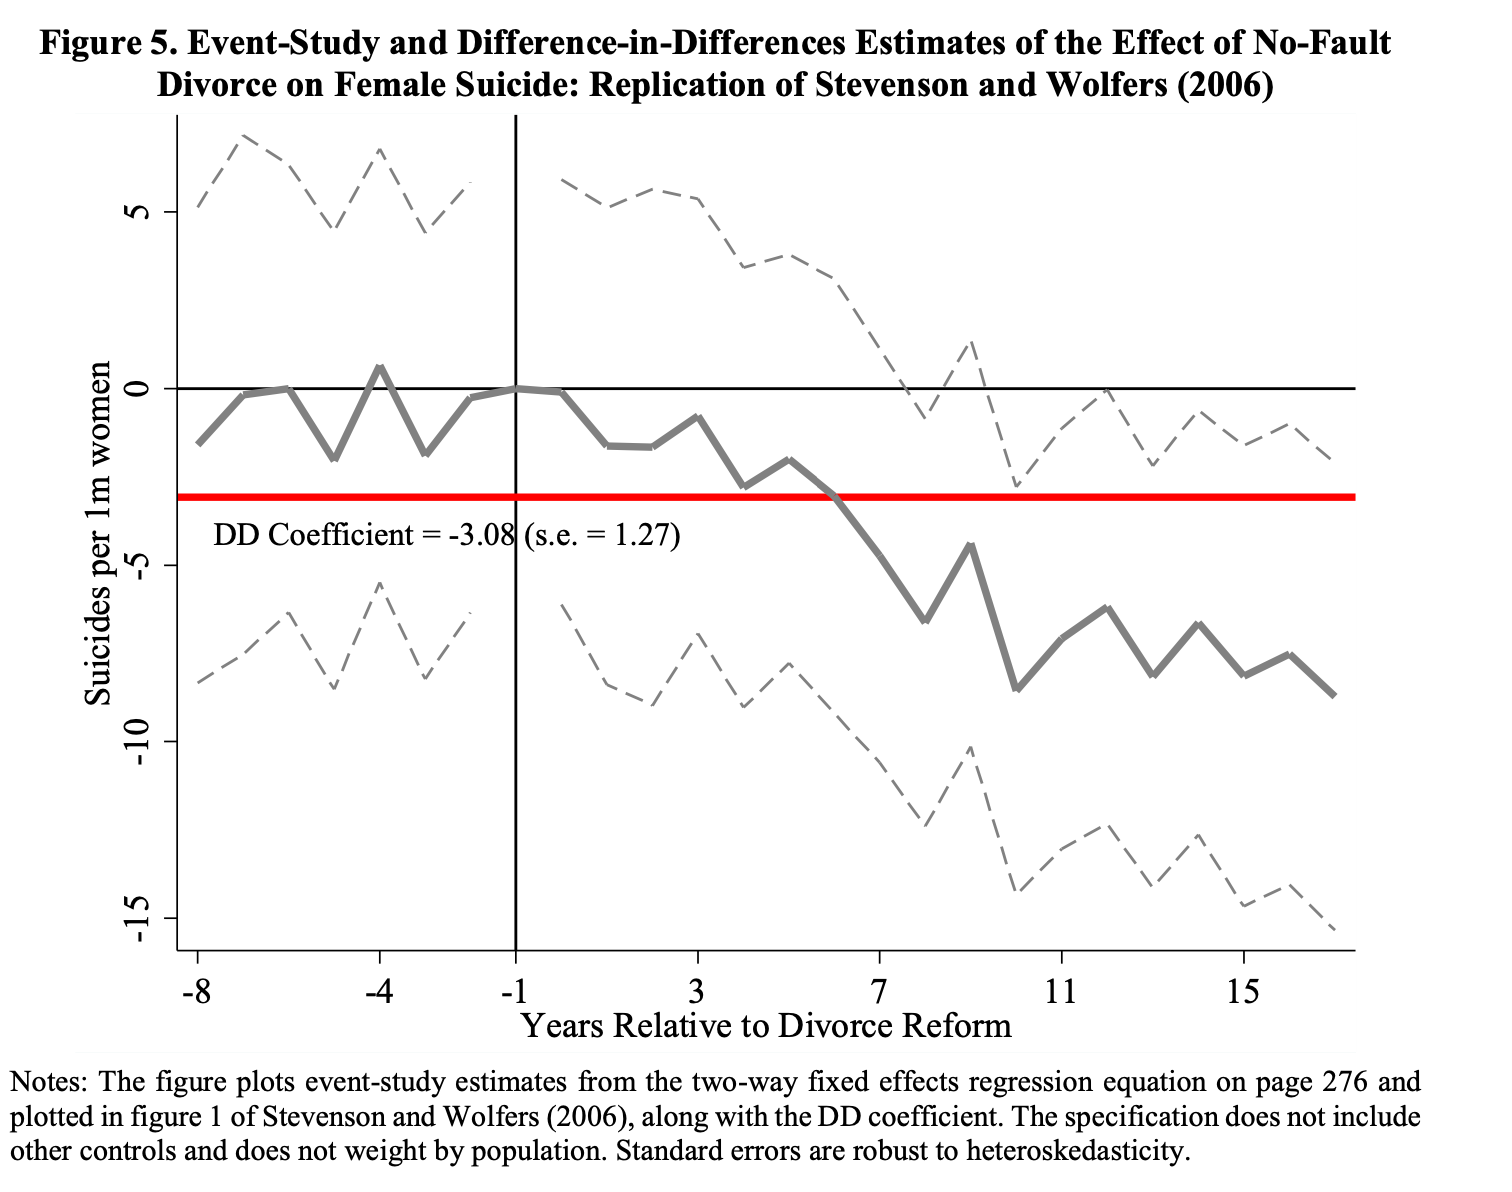
\includegraphics[height=0.9\textheight]{resources/gb_fig5.png}
\end{frame}

\begin{frame}{Decomposition Plot (Goodman-Bacon 2020)}
\centering
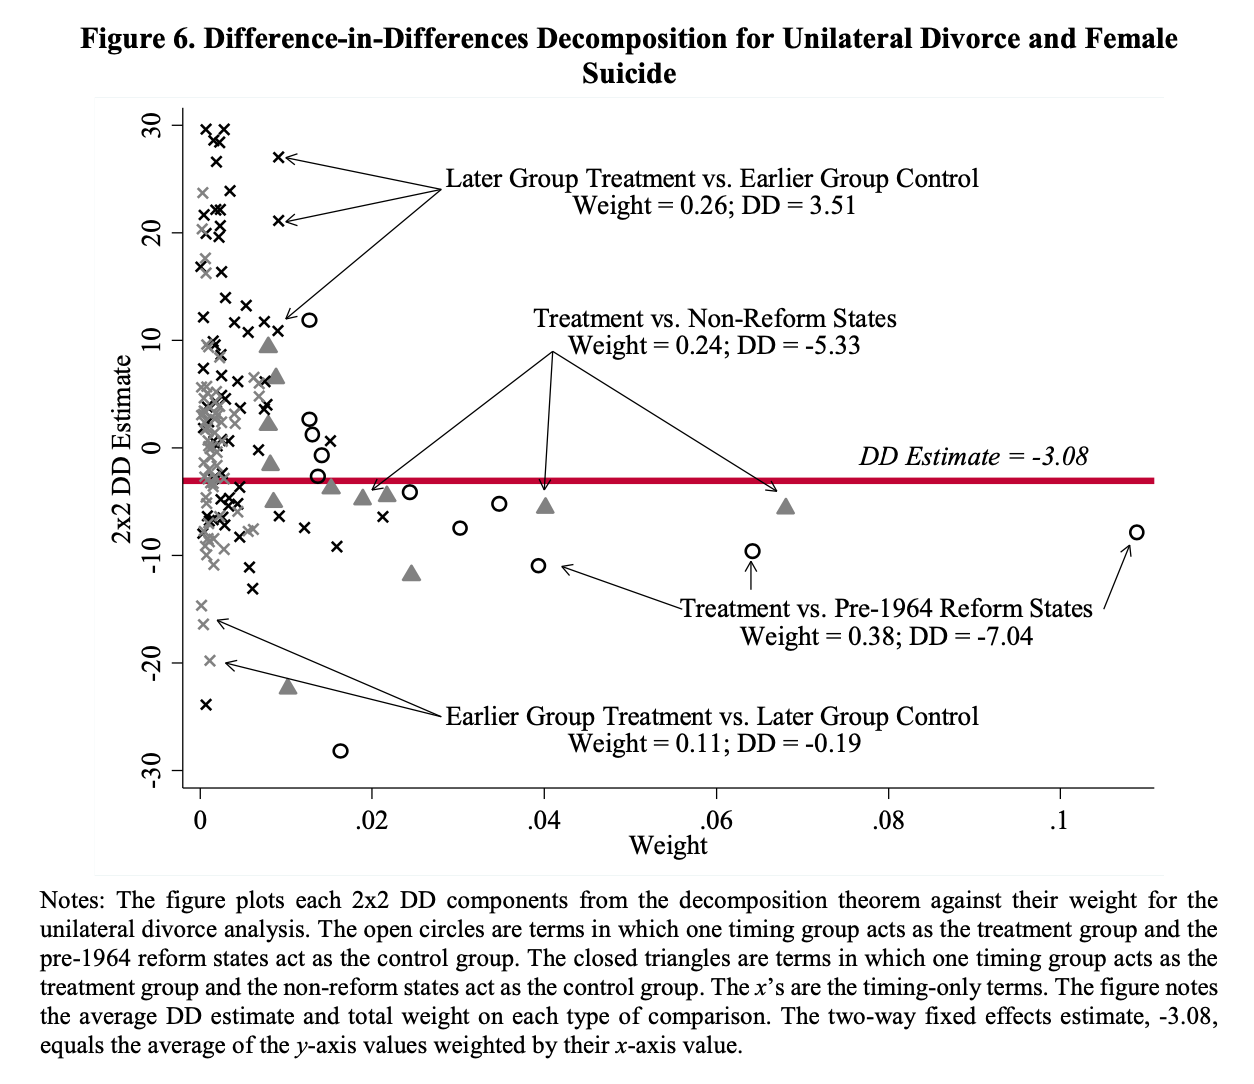
\includegraphics[height=0.9\textheight]{resources/gb_fig6.png}
\end{frame}

\begin{frame}{Application: Estimates (Goodman-Bacon 2020)}
\centering
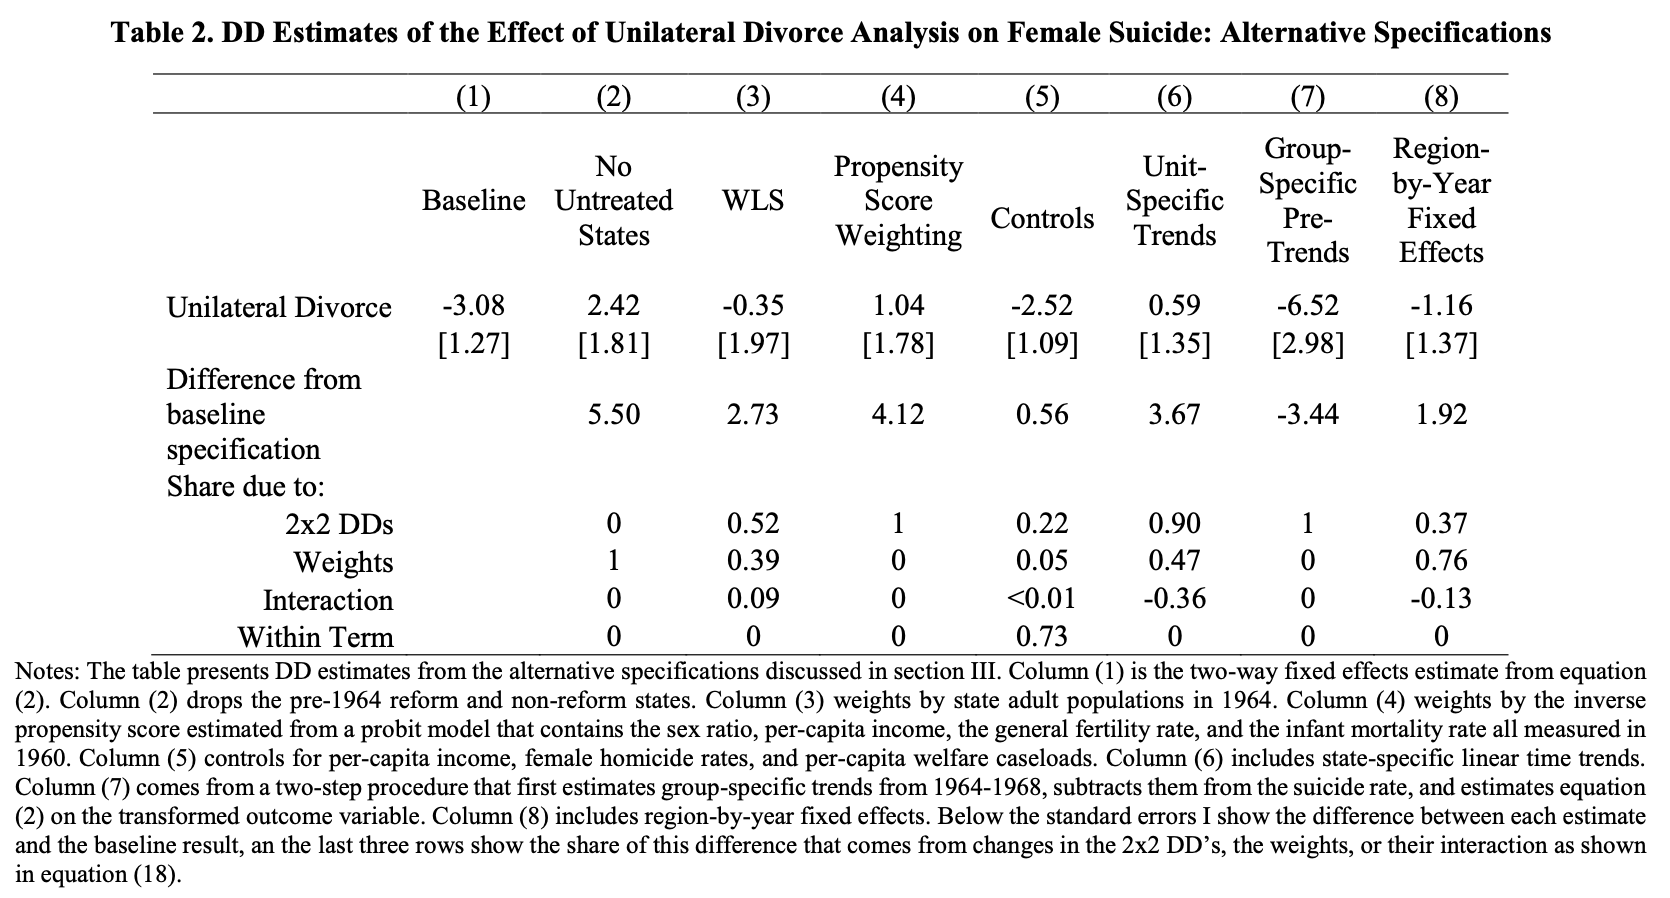
\includegraphics[height=0.9\textheight]{resources/gb_tab2.png}
\end{frame}


\begin{frame}{Recap}
\begin{itemize}
\item The Goodman-Bacon (2020) paper tells us what we \alert{are} measuring with TWFE.
\item Weird things can happen like \alert{negative weights}.
\item But it doesn't really tell us what we \alert{should do}.
\item Other than be careful and plot the \alert{event study} plot always.
\end{itemize}

\end{frame}



\section*{Callaway and Sant'Anna (2020)}
\begin{frame}{Some Theory}
Definitions
\begin{itemize}
\item $G_i$ when is $i$ treated (group/cohort).
\item $C_i$ set of never treated individuals
\item $Y_{it} = [G_i > t] Y_{it}(0) + [G_i \leq t] Y_{it}(G_i) $
\item Idea: multiple PO for $Y_{it}(z)$
\end{itemize}

Assumptions
\begin{itemize}
\item Irreversibility: $D_{it} \geq D_{i,t-1}$.
\item Modified Parallel trends for $t \geq g \text { and } s \geq t$:
\begin{align*}
\mathbb{E}\left[Y_{t}(0)-Y_{t-1}(0) \mid G=g\right]&=\mathbb{E}\left[Y_{t}(0)-Y_{t-1}(0) \mid C=1\right] \\
\mathbb{E}\left[Y_{t}(0)-Y_{t-1}(0) \mid G=g\right]&=\mathbb{E}\left[Y_{t}(0)-Y_{t-1}(0) \mid D_{s}=0, G \neq g\right]
\end{align*}
Can also do parallel trends \alert{conditional on covariates}.
\end{itemize}
\end{frame}

\begin{frame}{Grouped TE}
\small
All observations treated at time $g$ are grouped into a \alert{cohort}
\begin{align*}
ATT(t,g) = \mathbb{E}\left[Y_{t}(g)-Y_{t}(0) \mid G=g\right]
\end{align*}
We can estimate a \alert{time-varying} and \alert{cohort-specific} ATT using \alert{never-treated} or \alert{not-yet-treated}.
\begin{align*}
\operatorname{ATT}(g, t)&=E\left[Y_{t}-Y_{g-1} \mid G=g\right]-E\left[Y_{t}-Y_{g-1} \mid C=1\right] \\
\operatorname{ATT}(g, t)&=E\left[Y_{t}-Y_{g-1} \mid G=g\right]-E\left[Y_{t}-Y_{g-1} \mid D_{t}=0, G \neq g\right]
\end{align*}
In may be better to simply estimate and report these objects.\\
 (Assuming modified parallel trends hold).\\
 Unless you have lots of groups -- I would stop here.
\end{frame}


\begin{frame}{Combining Grouped TE}
We could average the $\operatorname{ATT}(g, t)$ and report those (if we have too many groups).
\begin{align*}
\theta_{S}(g)&=\frac{1}{\mathcal{T}-g+1} \sum_{t=2}^{\mathcal{T}} 1\{g \leq t\} A T T(g, t)\\
\theta_{S}^{O}&:=\sum_{g=2}^{\mathcal{T}} \theta_{S}(g) P(G=g)
\end{align*}
This is the \alert{time-average} for each group and the overall average resepectively.
\end{frame}

\begin{frame}{Combining Grouped TE}
We could also do the group-averaged \alert{event study}
\begin{align*}
\theta_{D}(e):=\sum_{g=2}^{\mathcal{T}} 1\{g+e \leq \mathcal{T}\} A T T(g, g+e) P(G=g \mid G+e \leq \mathcal{T})
\end{align*}
This combines cohorts and plots the average $k$ periods before and after treatment.
\end{frame}

\begin{frame}{Application: Estimates}
\centering
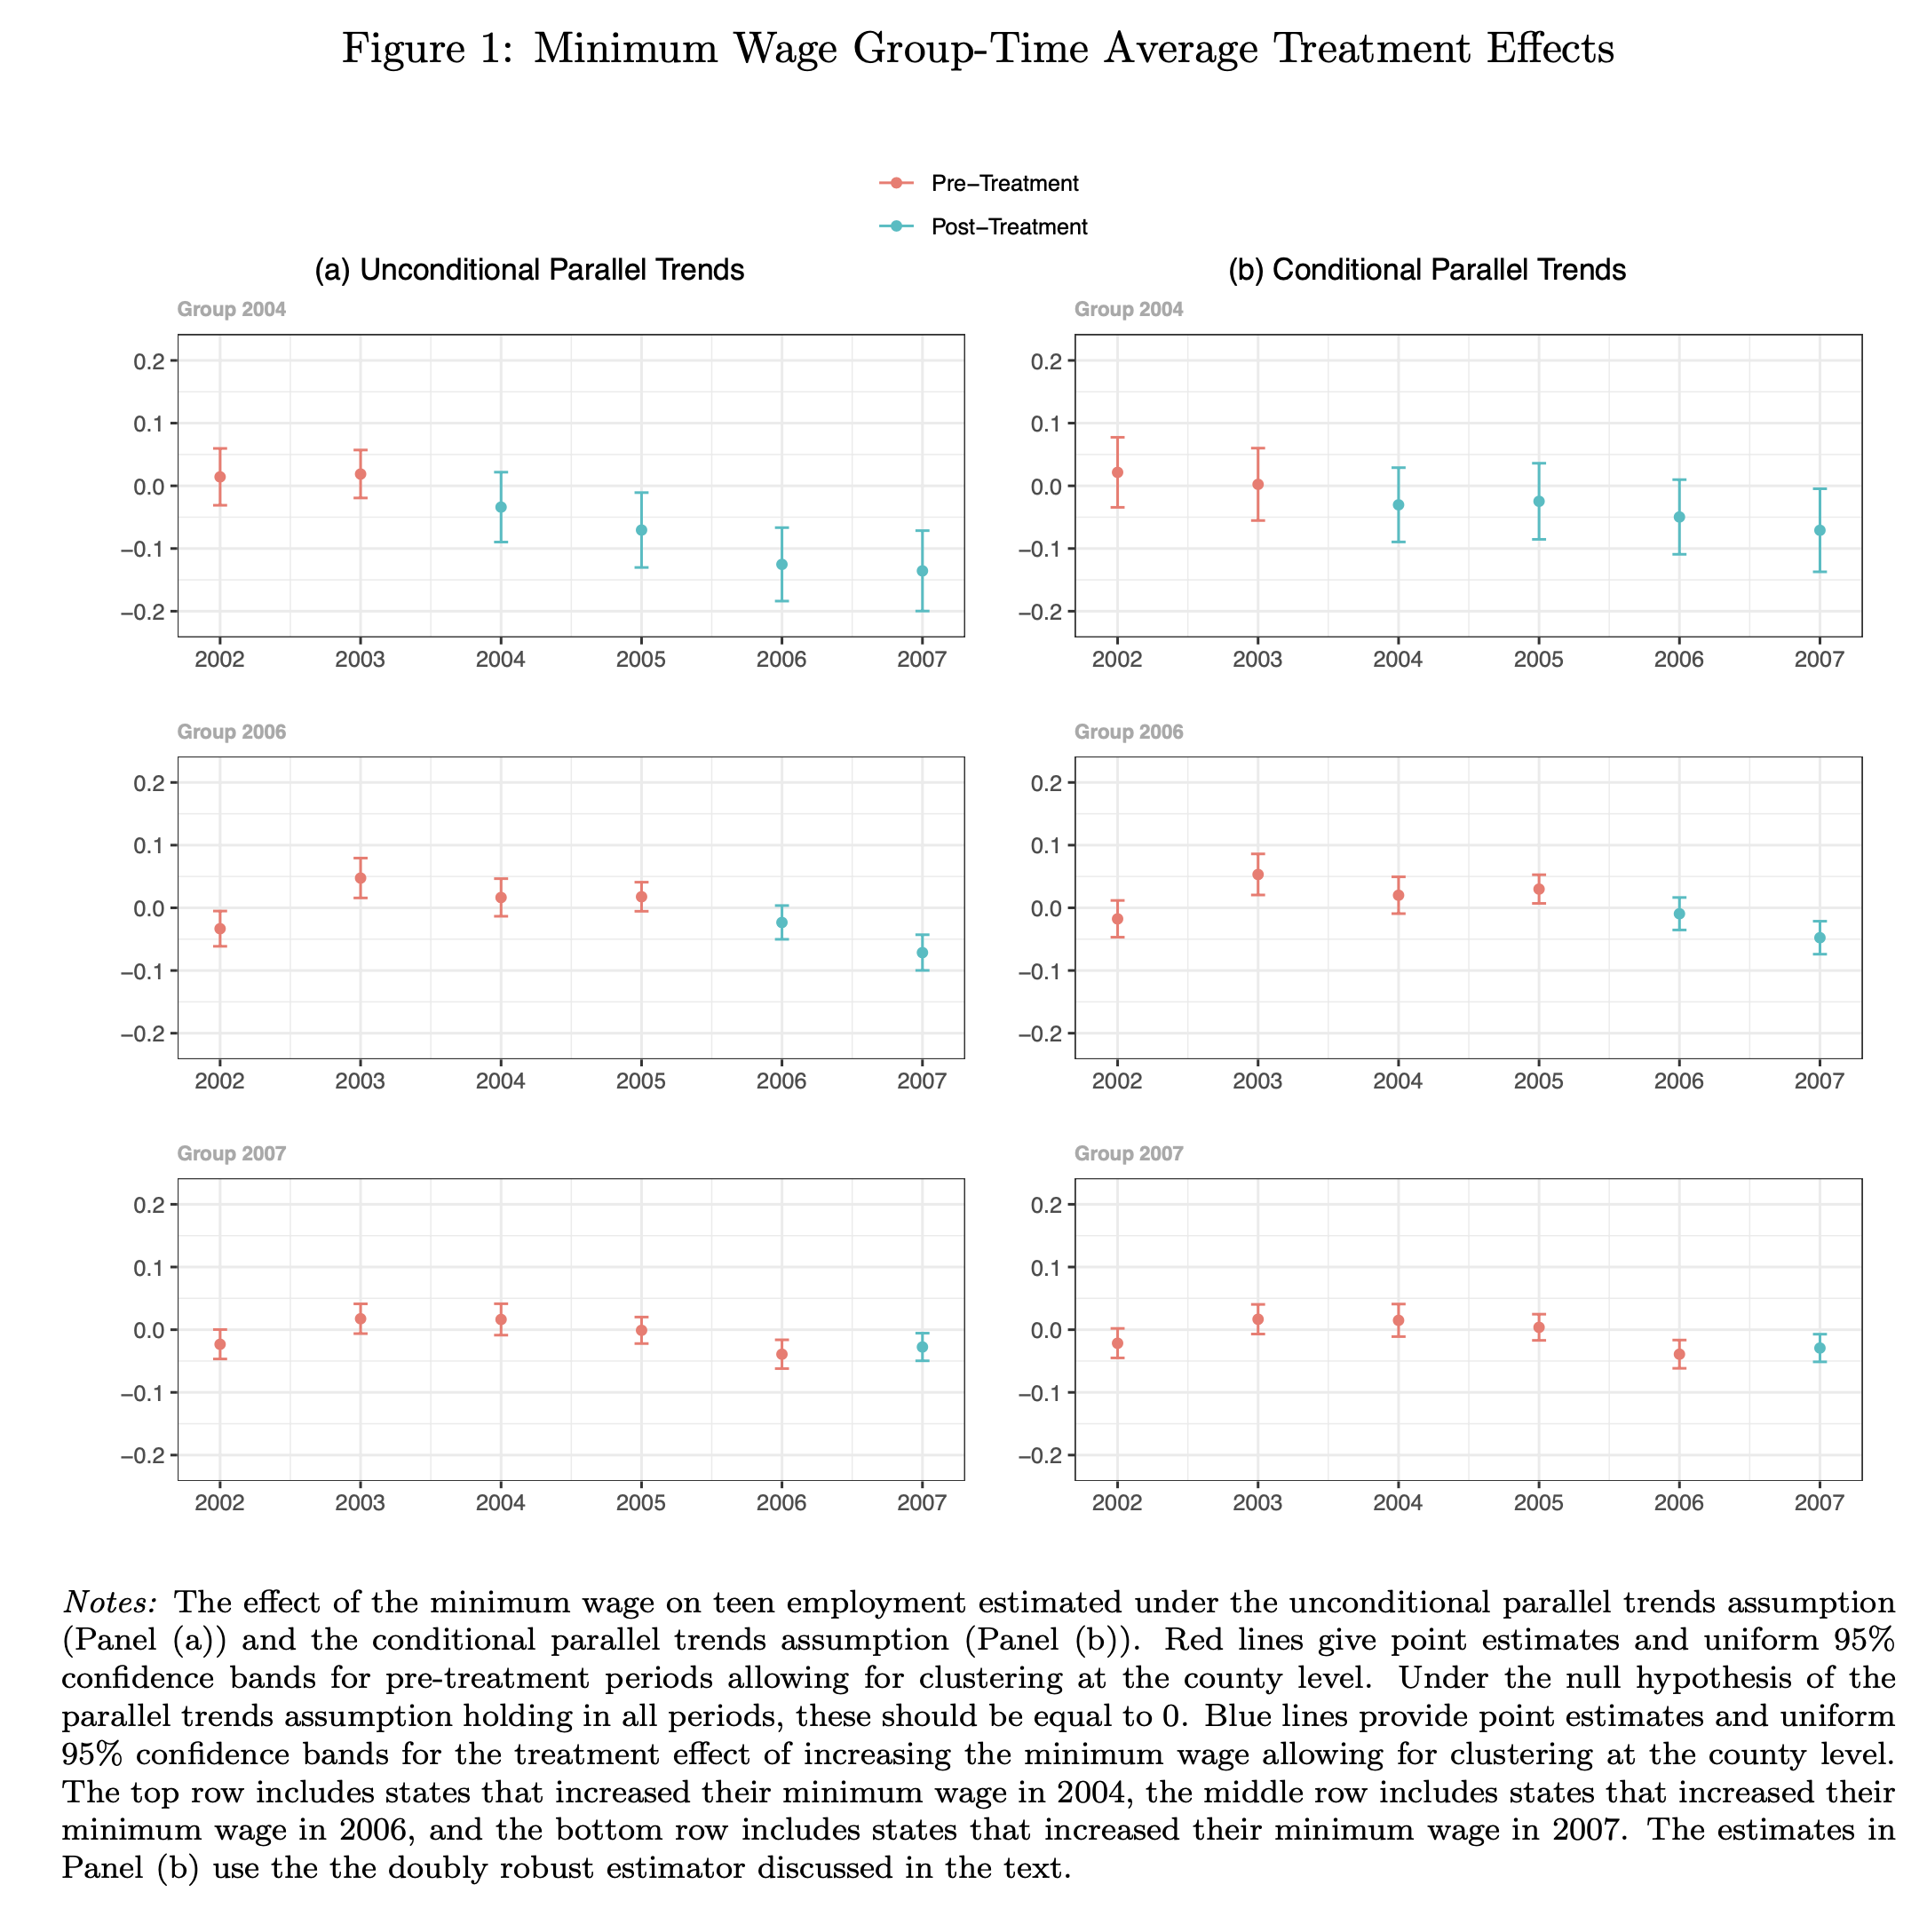
\includegraphics[height=0.9\textheight]{resources/csa_fig1.png}
\end{frame}

\begin{frame}{Application: Estimates}
\centering
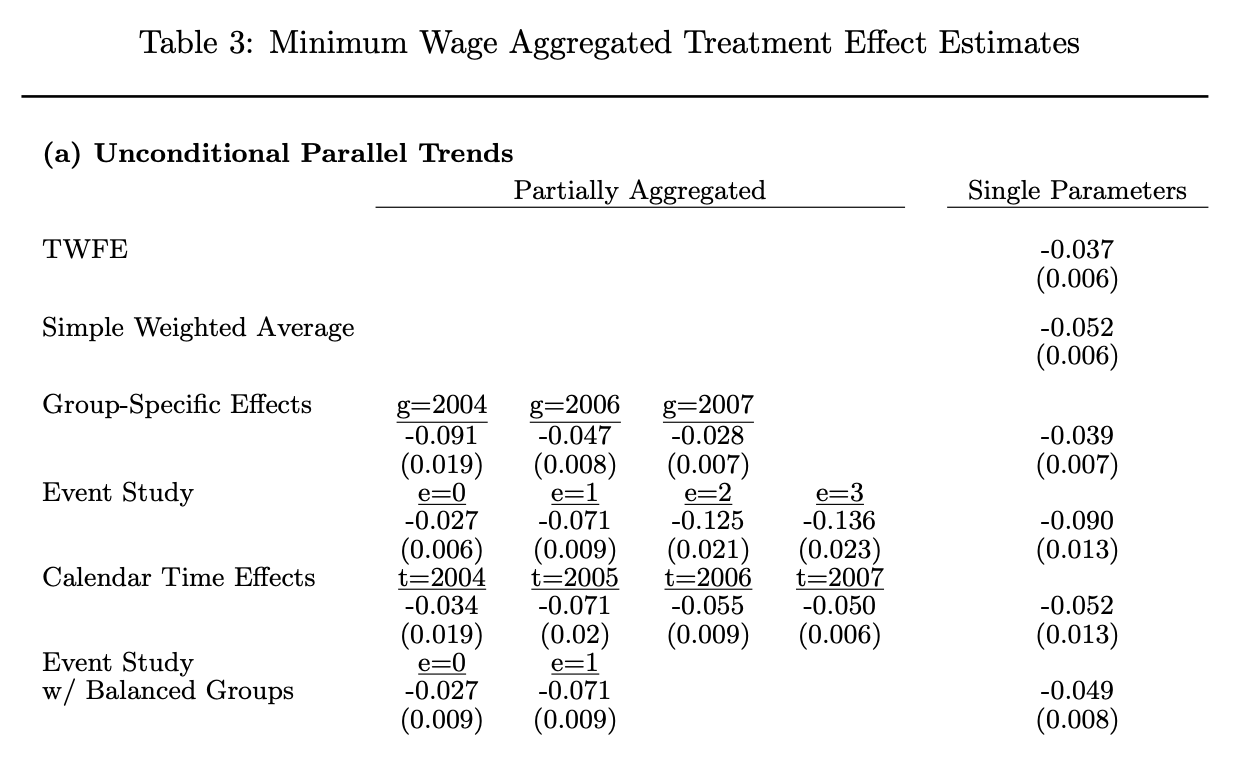
\includegraphics[height=0.9\textheight]{resources/csa_tab3a.png}
\end{frame}

\begin{frame}{Application: Estimates}
\centering
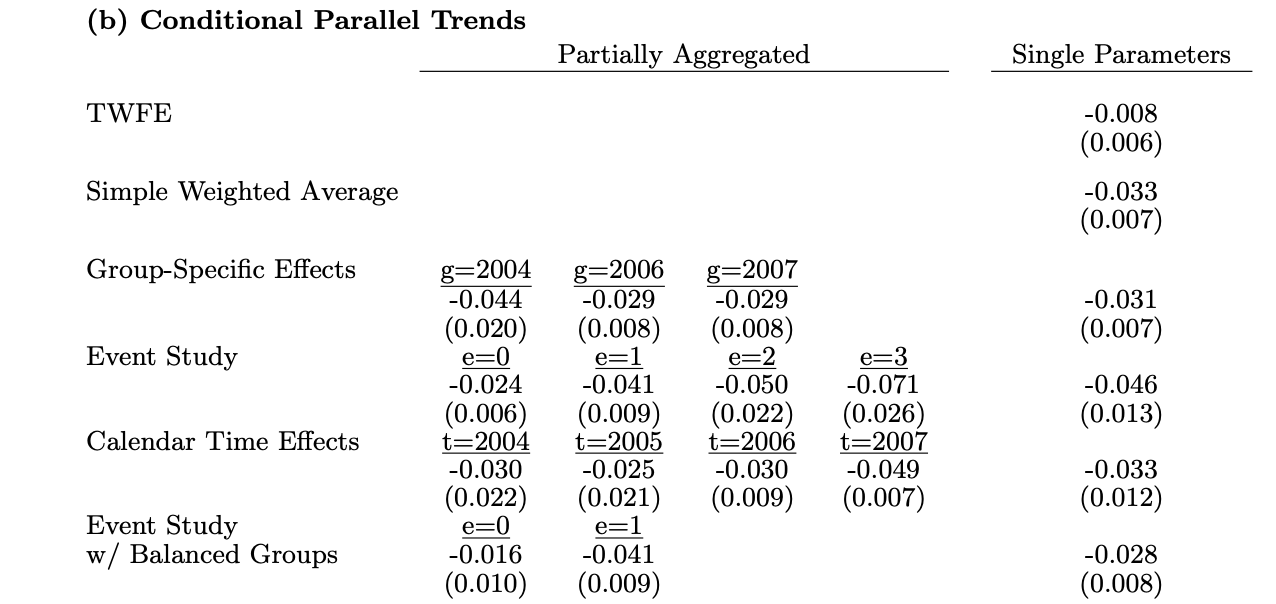
\includegraphics[height=0.9\textheight]{resources/csa_tab3b.png}
\end{frame}

\begin{frame}{Application: Estimates}
\centering
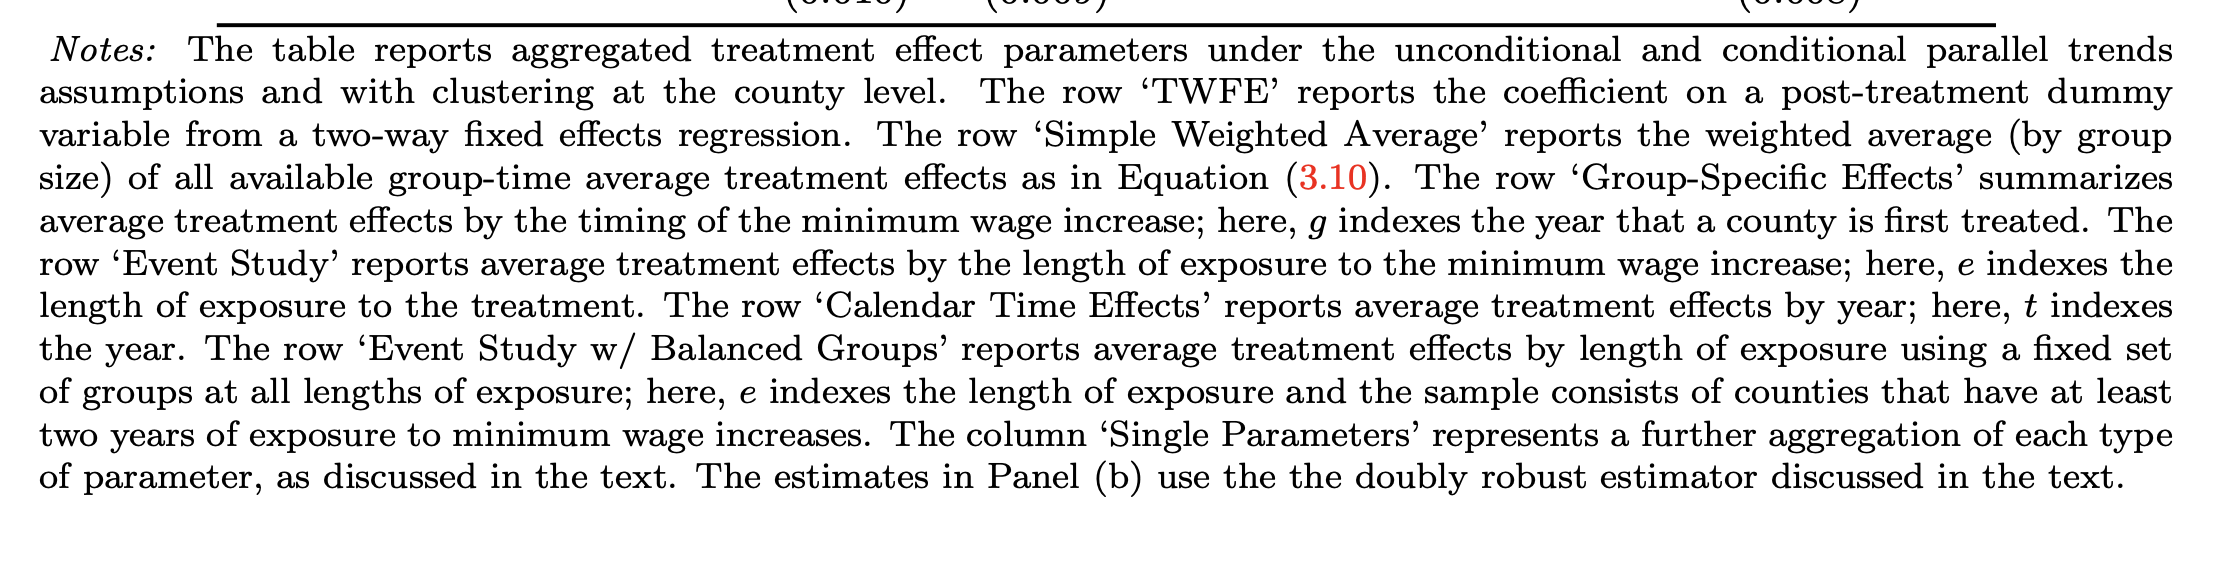
\includegraphics[width=\textwidth]{resources/csa_notes.png}
\end{frame}

\begin{frame}{Explore \texttt{did} in \texttt{R}}
\href{https://bcallaway11.github.io/did/}{https://bcallaway11.github.io/did}
\end{frame}

\section*{Thanks!}




\end{document}